\documentclass[25pt, a0paper, portrait]{beamer}

% ====================
% Packages
% ====================

\usepackage[T1]{fontenc}
\usepackage{lmodern}
\usepackage[size=a0]{beamerposter}
\usetheme{gemini}
\usecolortheme{ox}
\usepackage{graphicx}
\usepackage{booktabs}
\usepackage{tikz}
\usepackage{pgfplots}
\usepackage{commath}
\usepackage{wrapfig}
\usepackage{subcaption}
\pgfplotsset{compat=1.14}
\usepackage{anyfontsize}
\graphicspath{{./images/}}

% ====================
% Lengths
% ====================

% If you have N columns, choose \sepwidth and \colwidth such that
% (N+1)*\sepwidth + N*\colwidth = \paperwidth
\newlength{\sepwidth}
\newlength{\colwidth}
\setlength{\sepwidth}{0.025\paperwidth}
\setlength{\colwidth}{0.3\paperwidth}

\newcommand{\separatorcolumn}{\begin{column}{\sepwidth}\end{column}}

% ====================
% Title
% ====================

\title{Using Hopfield Networks to restore corrupted greyscale images}

% ====================
% Footer
% ====================

\footercontent{ \hfill \hfill
  Daniel Haywood}

% ====================
% Logo
% ====================
\logoleft{
\includegraphics[height=4cm]{logos/Imperial-college-white.png}}

% ====================
% Body
% ====================

\begin{document}



\begin{frame}[t]
\begin{columns}[t]
\separatorcolumn

\begin{column}{\colwidth}

  \begin{block}{An introduction to Hopfield Networks} \small

    \textbf{Hopfield Networks} are a form of Ising model that have many uses in various sectors: 
    computational neuroscience, optimisation, and more. Similar to an Ising model, they
    are comprised of an array of nodes that are given a \textit{magnetic spin},
    either $+1$ or $-1$, and connections, \textit{'weights'}, linking them.
    We can use this archetecture to \textit{'train'} the network on given sets of data,
    effectively \textit{'storing the memory'} of the data on the network.
    Then, we can recover the stored data by inputting a new set of data
    and \textit{'updating'} the network using the weights we obtained from training
    it on our sets of data.

    In this project, we will look specifically at their application in image processing: how it can
    be used to restore and discern between corrupted pixellated images. By training the network on
    a set of images, we can then input corrupted versions of the images into the network, and updating
    the network will yield an image that should hopefully resemble the orignal image to a good degree
    of accuracy.

  \end{block}

  \begin{block}{Basic definitions} \small

    We start by defining our $n$ node spins $V_i$, where $i \in \{0, 1, ..., n\}$.
    These nodes all have connections to other nodes, and this is denoted by
    $T_{ij}$, which represents the connection between nodes $i$ and $j$. We note that,
    $\forall i, j, T_{ij} = T_{ji}$. Further, $T_{ij} = T_{ji} = 0$ whenever
    nodes $i$ and $j$ are not connected, or when $i = j$.

    Like an Ising model, we \textit{'update'} the network given a set of spins by
    considering a threshold for each node, denoted by $U_i$. Then, we say:

    \begin{equation} \label{update_rule}
      V_i = \begin{cases} 
              +1, & \sum_{j}T_{ij}V_j > U_i \\
              -1, & \sum_{j}T_{ij}V_j \leq U_i
            \end{cases}
    \end{equation}

    This threshold vector could be defined specifically to influence how specific nodes
    tend to behave, but for the purposes of this project we will define the threshold
    vector to be the zero vector, that is, $U_i = 0, \forall i$.

    This update can either be done \textit{asynchronously} or \textit{synchronously}, for the former,
    each $V_i$ is updated individually and the new $V_i$ is used for the updates
    of other nodes, and for the latter, all updates use the initial set of node spins
    before any updates took place. If updating synchronously, some kind of internal
    clock or way to save previous states of the network must exist, and so most 
    biological systems, such as the brain, will update asynchronously.
  \end{block}

  \begin{alertblock}{The Hebbian learning rule} \small

    The core of the Hopfield network lies in its use in \textit{'storing'} states
    of the network to be recovered later. This is done using the \textit{Hebbian learning
    rule}. \cite{hopfield:1982}

    If we have a set of $m$ states $V^s, s \in \{1, ..., m\}$, we can use the
    Hebbian learning rule:

    \begin{equation} \label{hebbian_learning_rule}
      T_{ij} = \sum_{s}{V^s_i}{V^s_j}
    \end{equation}

    Since this equation yields nonzero values for the case where $i = j$, we must
    then adjust for this by resetting $T_{ij}$ to $0$ whenever $i = j$. This will 
    update the weights of the network and effectively \textit{'imprint'}
    the states into the network.

    Now we have our basic tools for applying a Hopfield network to our problem, we
    can start looking at basic uses of the network.
  \end{alertblock}

  \begin{block}{Maximum storage space} \small
    Naturally, Hopfield networks will get less and less accurate at recalling data as
    the amount of data increases. We use the concept of \textit{maximum storage space}
    to measure how many states the network can store before it is unlikely to be able to
    recall individual states.

    We can calculate the storage capacity of a network with $n$ nodes by using the following
    formula:

    \begin{equation} \label{recall_percentage}
      C \cong \frac{n}{2log_2n}
    \end{equation}

    Using this, we see that $C \approx 0.138n$. \cite{fncom:2017}

    Effectively, what this means is that for every $1000$ nodes in the network, approximately
    $138$ states can be recalled. For our application, since for an $n$-by-$m$ image there are
    $nm$ nodes in the network, we can store $0.138nm$ images with reasonable accuracy.

    Note that this means that the storage capacity is linear with the shape of the input,
    which for large sets of data is not preferable. Instead, to improve this, we can utilise a
    different learning rule, called the Storkey learning rule. \cite{storkey:1997}
  \end{block}

\end{column}

\separatorcolumn

\begin{column}{\colwidth}

  \begin{block}{Initialising and training the network} \small

    Suppose we have a set of $k$ $n$-by-$m$ uncorrupted images to train the model on,
    where each pixel can either be black or white.
    We can, without loss of generality, assign the colour black to the spin $+1$
    and white to $-1$. Now, each image can be represented as a set of $nm$ spins, 
    using each pixel as a node in the network, so we can use a Hopfield network to 
    store them.

    To set up our problem, we can store each image as a vector of its spins, so for
    the $s$th image:
    \begin{equation*}
      \boldsymbol{V^s} = \begin{bmatrix}
        V^s_1 \\
        V^s_2 \\
        \vdots \\
        V^s_{nm}
      \end{bmatrix}
    \end{equation*}

    Similarly, we also store the weights in an $nm$-by-$nm$ matrix:
    \begin{equation*}
      \boldsymbol{T} = \begin{bmatrix}
        T_{1,1}   & \dots   & T_{1,nm}\\
        \vdots      & \ddots  & \\
        T_{nm,1}  &         & T_{nm,nm}
      \end{bmatrix}
    \end{equation*}

    Then, we can apply the Hebbian learning rule to train the network on our images, using
    (\ref{hebbian_learning_rule}):
    \begin{equation} \label{hebbian_simple_eq}
      \boldsymbol{T} = \frac{1}{k} \sum_{s}(\boldsymbol{V^s}\otimes\boldsymbol{V^s} - diag({V^s_1}{V^s_1}, \dots, {V^s_{nm}}{V^s_{nm}}))
    \end{equation}
    where $\otimes$ indicates the vector outer product.

    This then gives us:
    \begin{equation*}
      \boldsymbol{T} = \frac{1}{k} \sum_{s} \begin{bmatrix}
        0                 & {V^s_1}{V^s_2}  & \dots   & {V^s_1}{V^s_{nm}}\\
        {V^s_2}{V^s_1}    & \ddots          &         & \vdots \\
        \vdots            &                 &         & \vdots \\
        {V^s_{nm}}{V^s_1} & \dots           & \dots   & 0
      \end{bmatrix}
    \end{equation*}
    as desired.

  \end{block}

  \begin{block}{Restoring images} \small

    Now that the network has been trained on the images, we can use it to restore
    corrupted images. To do this, we take the matrix $\boldsymbol{T}$ that we
    recieved from training and an input state $\boldsymbol{V}$, which represents
    our image to be restored.

    By updating the state using (\ref{update_rule}), we recieve a new image back,
    which we can then interpret again as an image. This will be our restored image.

    We can test our trained system by inputting our orignal images as well as our
    corrupted ones. $\boldsymbol{V}^s$:
    
    \begin{figure}[ht]
      \subcaptionbox*{Testing on uncorrupted images}[.3\linewidth]{%
        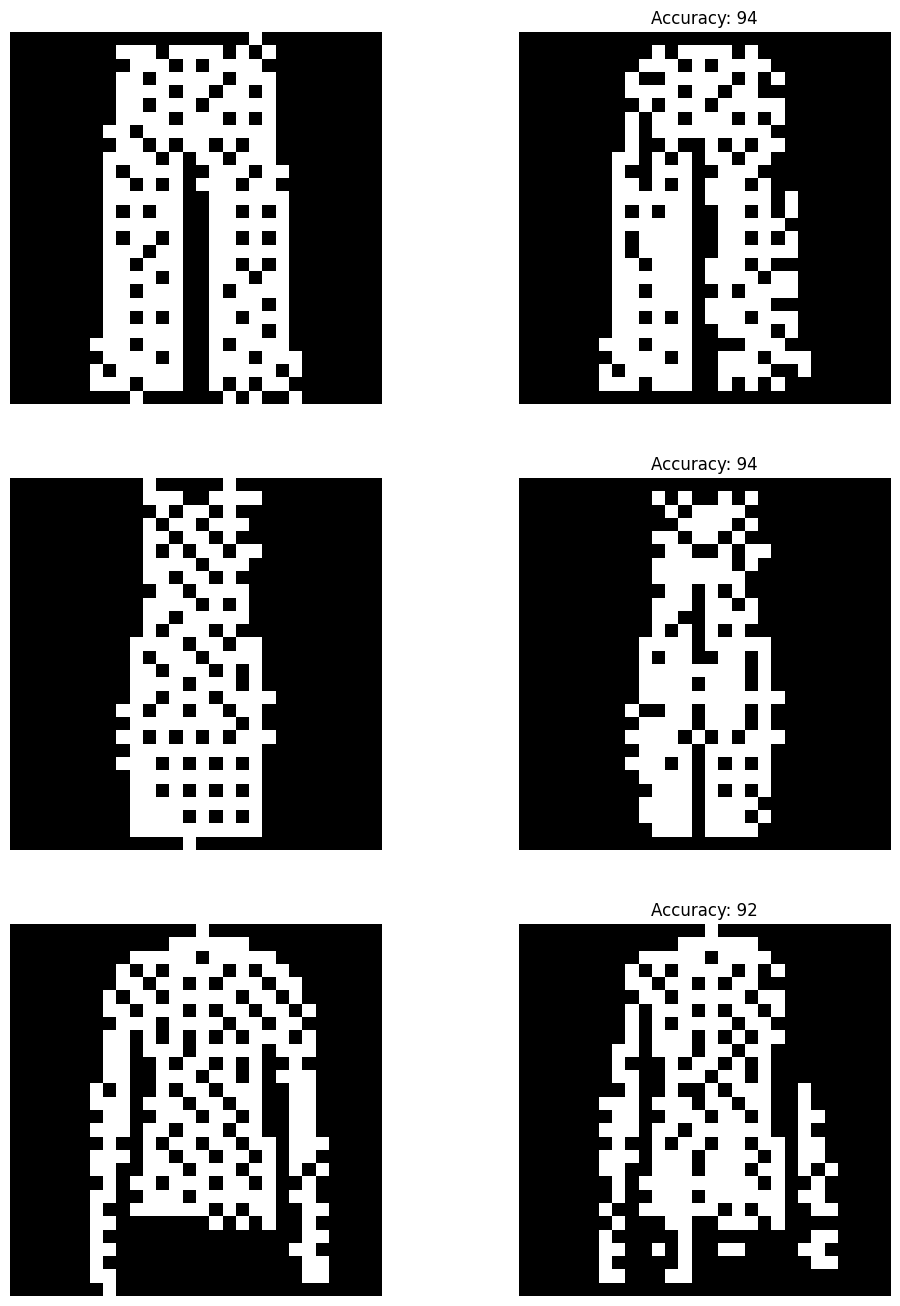
\includegraphics[width=\linewidth]{bwoutput}%
      }%
      \hfill
      \subcaptionbox*{Inputting  corrupted equivalents}[.3\linewidth]{%
        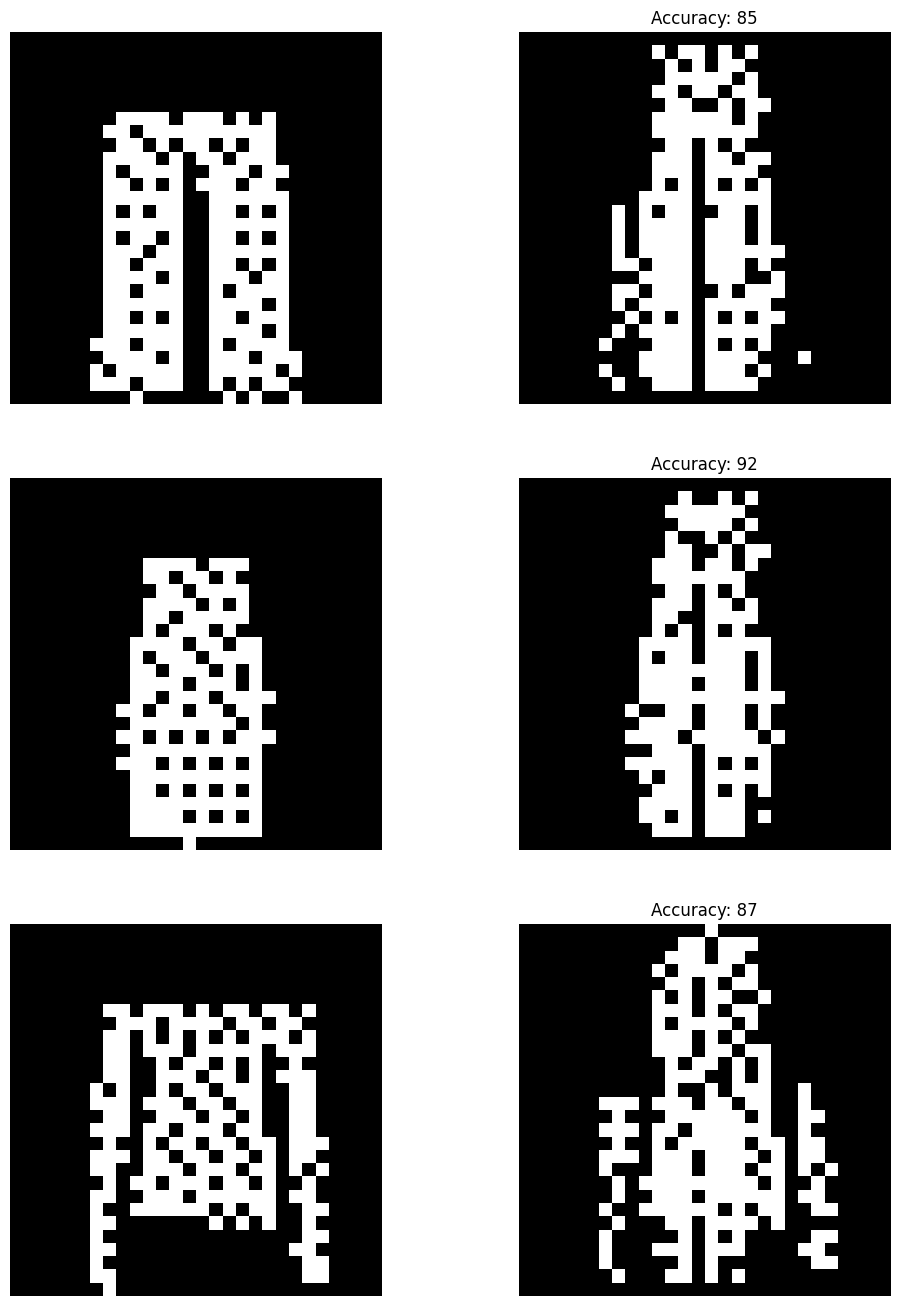
\includegraphics[width=\linewidth]{bwoutput2}%
      }
      \caption{Testing our network}
    \end{figure}

    Here, we see that the model is able to distinguish between the various images to
    a relatively high degree of accuracy, around $90\% - 95\%$. While it is not perfect, it
    can tell the difference between the images, and the updated images are still
    recognisable, despite them all looking relatively similar to each other. Training on
    more images should still produce good results, since as long as we stay below the
    maximum storage capacity of $0.138nm$, we can store more memories in the network.
    In our particular case, since the images are $28$-by-$28$, as we are using the
    \texttt{fashion-mnist} dataset, so the maximum number of images we can store is
    around $108$.

    We also see that when inputting corrupted images, which we obtained by masking the
    top $6$ lines of the image, that it is somewhat able to recover the image.
    We are able to recover the image to an accuracy of $85\%$ to $95\%$. The recovery
    accuracy of images depends greatly on the images themselves, and since these images
    are particularly similar, since they are all clothing items, it is not able to recover
    them perfectly. In this sense, for these types of images a Modern Hopfield network,
    which are Hopfield networks which have been adapted so the storage capacity is no longer
    linear with the input shape, would be preferable. \cite{ramsauer:2021}

  \end{block}

\end{column}

\separatorcolumn

\begin{column}{\colwidth}

  \begin{block}{Moving to greyscale images} \small

    What if instead of just working with spins of $+1$ or $-1$, we were to work
    with spins that take continuous values? We would be able to express a continuum
    of values for each pixel, instead of just black or white.

    To do this, we instead model the spin as being a complex number of the form $e^{i\theta}$,
    with $0 \le \theta \le \pi$. This includes the values $+1$ and $-1$, which will still
    represent the colours black and white respectively, but we can model the pixels
    as any colour on the greyscale.

    To get this working with our model, we need to adjust some of our rules:

    \heading{New update rule}

    Since we are now working with continuous values, it doesn't make sense to have a threshold
    value anymore. Instead, we just take the weighted average of all of the connected pixels,
    and renormalise the complex value so its modulus is $1$.

    \begin{equation} \label{complex_update_rule}
      V_i = \frac{\sum_{j}T_{ij}V_j}{\norm{\sum_{j}T_{ij}V_j}}
    \end{equation}

    This will inevitably move all of the pixels closer to grey, but we will adjust for that later.

    \heading{New learning rule}

    We also need to change the learning rule, as we can't check for a change in sign anymore.
    Instead, we calculate the distance between each pixel's colour by using its argument, and
    scaling it so that a weight of $-1$ represents the pixels being as far away as possible,
    and $1$ represents the pixels being the same.

    So, for any given state $s$,

    \begin{equation*}
      a^s_{ij} = \abs{arg(\frac{V^s_i}{V^s_j})}
    \end{equation*}

    is the angle between $V^s_i$ and $V^s_j$. Now, we use this to form our new learning rule:
    
    \begin{equation} \label{complex_learning_rule}
      T_{ij} = \sum_{s}(1 - \frac{2a^s_{ij}}{\pi})
    \end{equation}

    Again, we set $T_{ij}$ to equal $0$ whenever $i = j$. Now the ground rules are in place
    for our new network, we can test it out on some greyscale images.

  \end{block}

  \begin{block}{Training and restoration of greyscale images} \small

    Using the same method as before, we get the pixels' values, and scale them to be on the
    complex unit circle with positive imaginary part. Then, we use these as our node spins and
    train the network on them using (\ref{complex_learning_rule}), 

  \end{block}

  \begin{block}{References}
    \footnotesize{\bibliographystyle{plain}\bibliography{refs}}

  \end{block}

\end{column}

\separatorcolumn
\end{columns}
\end{frame}

\end{document}